\documentclass{article}
\usepackage[usenames,dvipsnames]{xcolor}
\usepackage{tikz}
\tikzset{mygrid/.style={thick,color=#1!50},
         mygrid/.default=black,
         roundnode/.style={circle,draw=black,fill=blue!20}}

%\usetikzlibrary{intersections}
%\usetikzlibrary{arrows}
%\usetikzlibrary{arrows.meta}
\usetikzlibrary{decorations.pathmorphing}
%\usetikzlibrary{fit}
\usetikzlibrary{calc}
%\usetikzlibrary{through}
%\usetikzlibrary{positioning}
\usetikzlibrary{graphs}
\usetikzlibrary{mindmap}
%\usetikzlibrary{backgrounds}


\pgfdeclarelayer{background}
\pgfdeclarelayer{alpha}
\pgfdeclarelayer{beta}
\pgfsetlayers{background,main,alpha,beta}



\parindent=0pt

\begin{document}
\list{--}
\item This is pgf version \pgfversion{}.
\item This Use \textbf{foreach} to do: \foreach \x in {1.5,2.5,...,9.5} {\x{}  } or \foreach \x/\y in {1/2} {$x=\x,y=\y$}
\endlist
\begin{center}
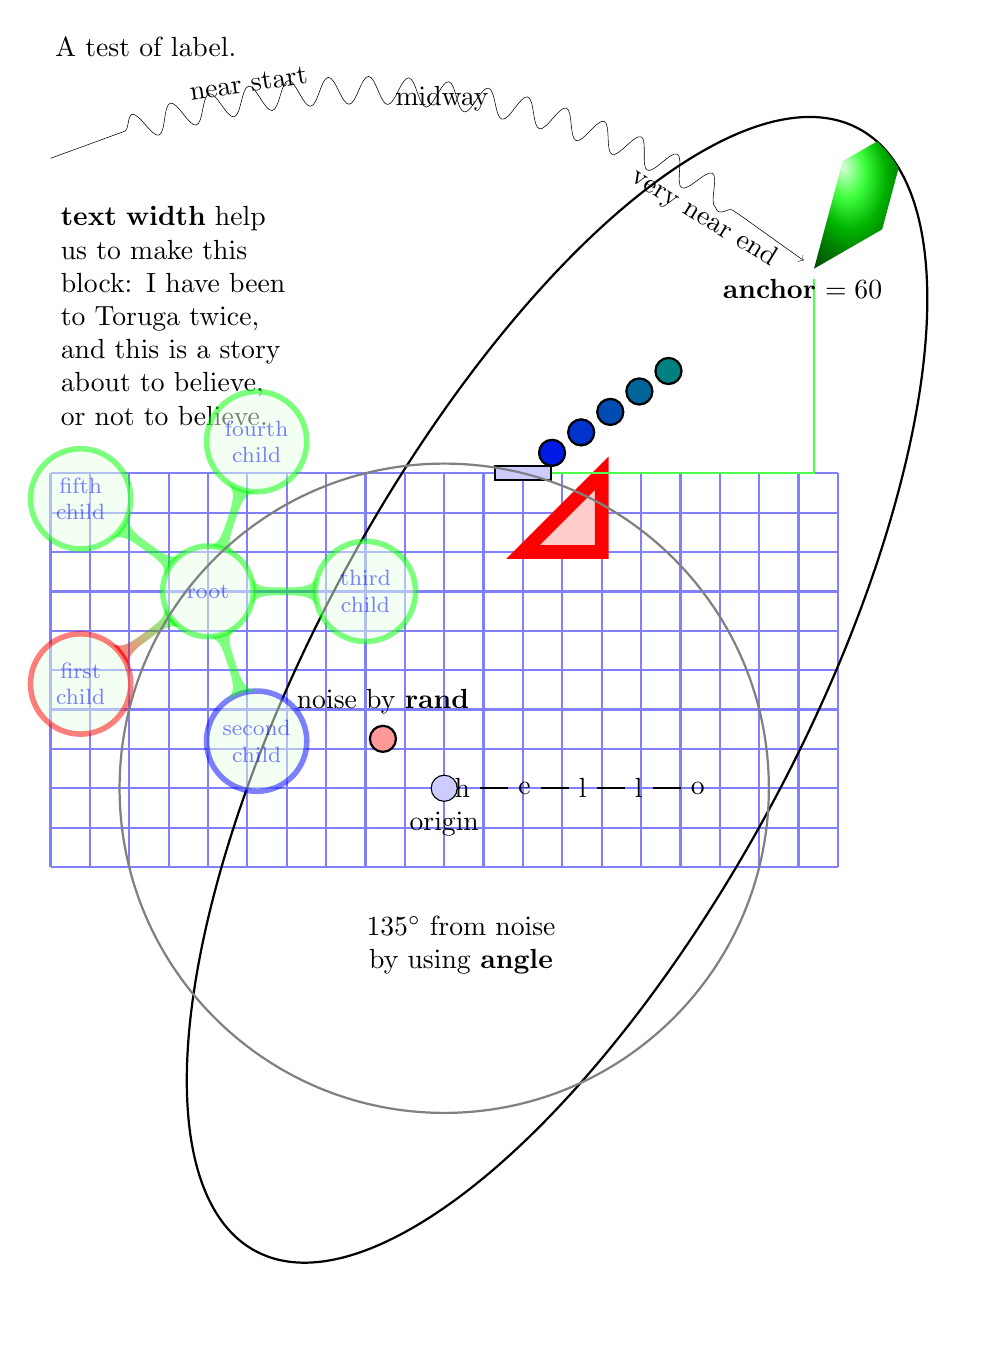
\begin{tikzpicture}[thick]
\coordinate (origin) at (0,0);
\draw[step=0.5,mygrid=blue] (-5,-1) grid (5,4);
\node[right,text width=3cm] at (-5,6) {\textbf{text width} help us to make this block: I have been to Toruga twice, and this is a story about to believe, or not to believe.};
\begin{scope}[shift={(1,1)},rotate=30,xslant=1]
\clip[draw] (0,0)++(0.5,0) circle [radius=5];
\shade[ball color=green] (3,3) node (a){} rectangle +(1,1);
\end{scope}
\filldraw[fill=red!20,draw=red,line width=5pt] (1,3) -- ++(1,0) -- +(0,1) -- cycle;
\node[rectangle,draw,fill=blue!20,inner sep=0,minimum height=5pt, minimum width=20pt] (let) at (60:2 |- 0,4) {} ;
\draw[green!70] (a) |- (let);

%%grow cyclic requires mindmap package
%%while grow=rigt does not
\begin{scope}[small mindmap, 
every node/.style={concept, execute at begin node=\hskip0pt,fill=green!10,minimum size=5pt,text width=7ex,text=blue},
grow cyclic, concept color=green,
level 1/.style={sibling angle=72,level distance=2cm},
opacity=0.5]
\node at (-3,2.5) {root}
 child[concept color=red] { node{first child} }
 child { node[concept color=blue]{second child} }
 child { node{third child} }
 child { node{fourth child} }
 child { node{fifth child} };
\end{scope}

%%decorate needs decorations.pathmorphing package
\draw[->,decorate,decoration={snake,amplitude=5pt,segment length=0.5cm,pre length=1cm,post length=1cm},very thin] (-5,8) to [bend left] 
node[near start,sloped,above,label=above:A test of label.] {near start}
node[very near end,sloped, below] {very near end}
node{midway} (a);
\node[node distance=3cm, anchor=60,node distance=3] at (a) {\textbf{anchor} $=60$};

%%Need calc library
\node[roundnode,fill=red!40,auto,label=noise by \textbf{rand}] (noise) at ($ (180*rand:1) $) {};
\draw[gray] let \p1=($ (let) $),\n1={veclen(\x1,\y1)} in (origin) circle (\n1);
\foreach \d in {1,2,...,5} {\node[roundnode,fill=green!\d0!blue] at ($ (let)!0.\d!(a)$) {};}
\node[align=center] at ($(origin)!2!135:(noise)$) {$135^\circ$ from noise\\by using \textbf{angle}};

%%graphs package needed
\graph[grow right sep] {h -- e -- l -- l2/l -- o};



\begin{pgfonlayer}{beta}
\node[roundnode,label=below:origin] at (origin) {};
\end{pgfonlayer}

\end{tikzpicture}
\end{center}

%%TaiJi
\begin{center}

\begin{tikzpicture}[thick,yi/.style={circle,minimum size=0.5cm}]
\shade [draw=black] (0,0) circle [radius =3];
\shade [top color=black, bottom color=black!50,draw=black] (0,-3) arc [radius=3, start angle=-90, end angle=90]
arc [radius=1.5, start angle=90, end angle=270]
arc [radius=1.5, start angle=90, end angle=-90];

\node [yi,draw=black,fill=black] at (0,-1.5) {};
\node [yi,draw=white,fill=white] at (0,1.5) {};
\end{tikzpicture}
\end{center}

%%2015NewYear
\begin{center}
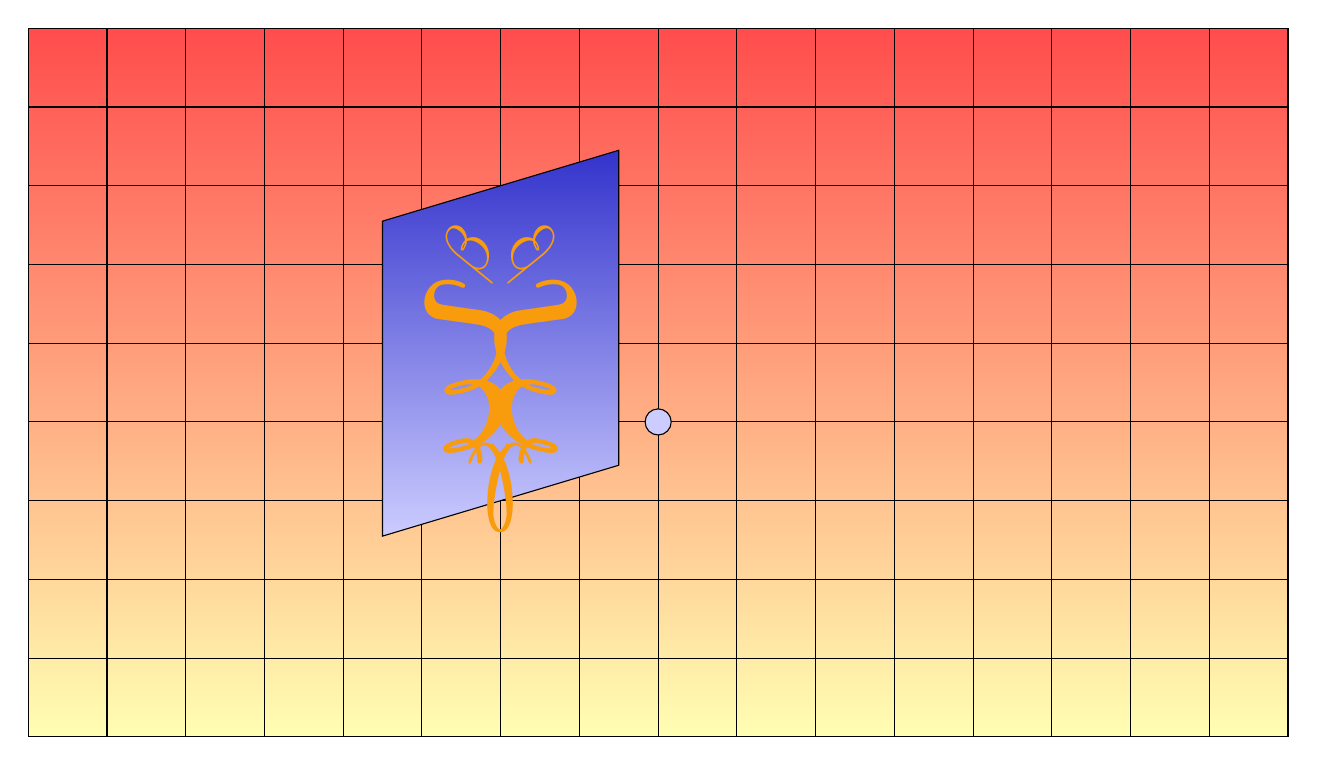
\begin{tikzpicture}
\shade [top color=red!70, bottom color=yellow!30] (-8,-4) rectangle (8,5);
\draw [step=1, black, thin] (-8,-4) grid (8,5);
\node [circle, draw] (goatmid) at (-2,1) {};
\filldraw[draw=black, shade, top color=blue!60!gray, bottom color=blue!20,yslant=0.3] (goatmid)++(-1.5,-2) rectangle +(3,4);

\foreach \x in {1,-1}
{
\begin{scope}[yellow!60!red,xscale=\x,scale=1.5,transform shape]
\node[yscale=-1,xshift=-0.75cm,rotate=13,scale=5,right] at (goatmid) {$\xi$};
\node[shift={(-0.4cm,0.4cm)},rotate=65,scale=1.7,right] at (goatmid) {$\beta$};
\node[yscale=-1, yshift=1.2cm,scale=3,rotate=25] at (goatmid) {$\ell$};
\end{scope}
}


\node[roundnode] at (0,0) {};
\end{tikzpicture}
\end{center}
\end{document}
%%\draw=\path[draw]
%%\clip=\path[clip]
%%\graph=\path[graph]
%%bend right ~ bend right=30 ~ in,out=right30, left 30
%%(left:2)=(180:2)
%%left ~ anchor=east ~ anchor 0
%For updating 2.10 to 3.0.0
%after moving the folder, it requires 
%sudo texhash 
% to make it work.
